\chapter{Architecture logicielle}

Notre projet peut être découpé en plusieurs modules comme montré précédemment.
L’architecture de notre logiciel va donc s’appuyer sur cette structure
modulaire. Chaque module sera relié aux autres par une interface centrale
recoupant les fonctionnalités de chaque module.
Le projet se présente sous la forme d’un programme, principalement écrit en Scala.
Par la suite, tous les éléments décrits seront considérés comme écrits en Scala,
et pour toute exception le langage utilisé sera précisé.

\section{Description des modules}

\subsection{Préparation des données}

Le module de préparation des données est divisé en trois parties représentées
sur la figure 11.

\paragraph{}

\begin{mdframed}[frametitle={Figure 11 : Diagramme de classes de la partie préparation des données}, innerbottommargin=10]
\begin{center}
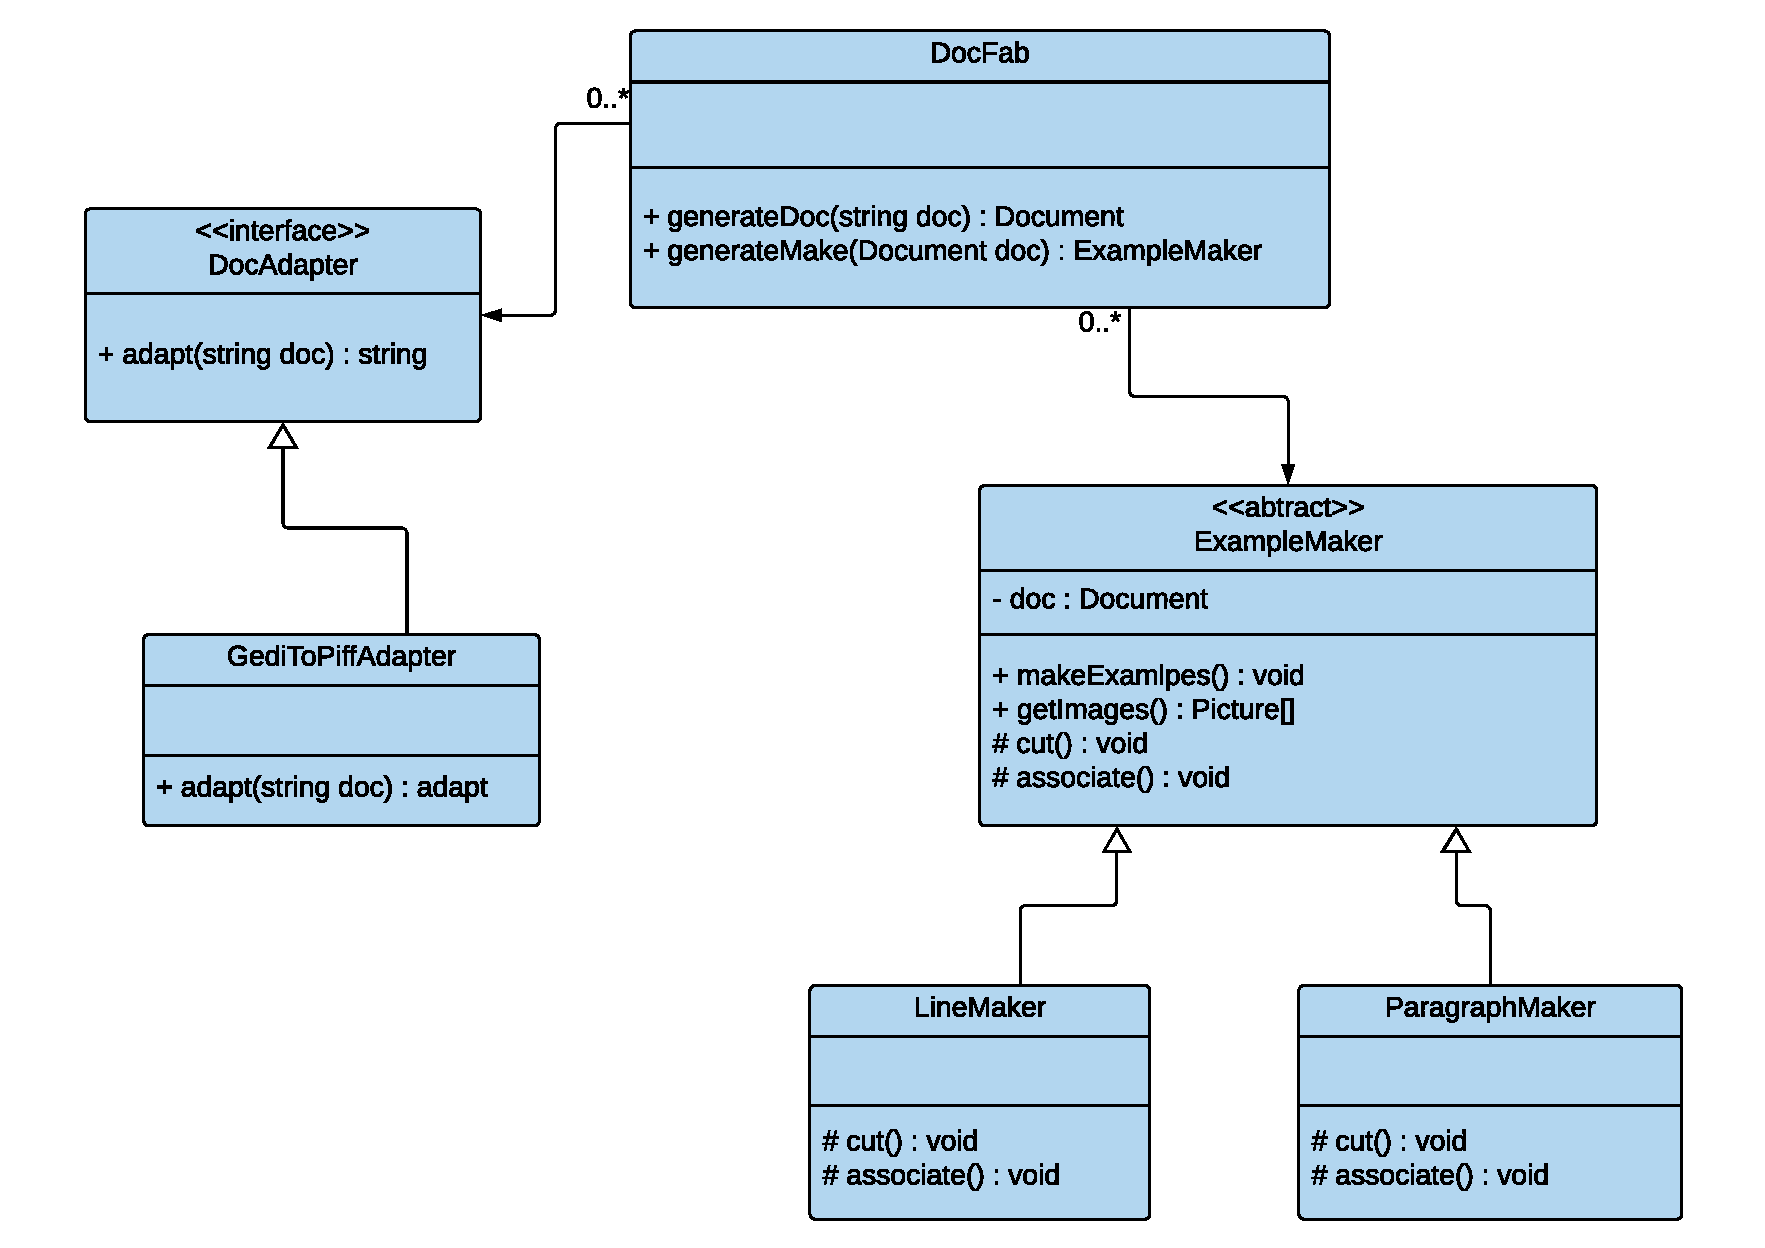
\includegraphics[scale=0.5]{prepa-data.pdf}
\end{center}
\end{mdframed}

\paragraph{}

La première est  une interface \textbf{DocAdapter} qui symbolise les
convertisseurs de formats vers PiFF. Nous en implémenterons un, la classe
\textbf{GEDIToPiFFAdapter}, afin de nous permettre de traiter comme prévu les
documents de la base Maurdor, présentée dans le précédent rapport. Grâce à
l’utilisation d’une interface, les développeurs sont cependant libres d’en
ajouter à l’avenir.

\paragraph{}

La seconde partie est une classe abstraite \textbf{ExampleMaker} permettant
la création des exemples d’apprentissage. En effet, les exemples peuvent être
créés selon plusieurs méthodes de détection de lignes et de découpe d’images :
par lignes ou par paragraphes. C’est pourquoi nous avons créé deux classes
\textbf{LineMaker} et \textbf{ParagraphMaker}, mais une potentielle troisième
méthode de détection de lignes à l’avenir pourra facilement être ajoutée à
notre logiciel, en créant une troisième classe héritière
d’\textbf{ExampleMaker}.

\paragraph{}

La troisième et dernière partie de ce module est une fabrique appelée
\textbf{DocFab} sur la figure 6 qui utilise les deux parties présentées
auparavant afin de créer des objets de type Document à partir d’une image et
des données du fichier d’entrée.

\paragraph{}

Par ailleurs, les fonctions de manipulation d’images utiliseront la bibliothèque graphique OpenCV, que nous avions déjà sélectionnée auparavant.

\subsection{Stockage des données}

\subsubsection{Choix du type de modélisation}

Concernant le stockage des données, nous avions plusieurs choix :
\begin{itemize}
\item écrire dans des fichiers ;
\item installer une base de données sur un serveur distant ;
\item installer une base de données sur un serveur local à la machine ;
\item installer une base de données sans serveur, en interne au logiciel.
\end{itemize}

\paragraph{}
Pour éviter d’utiliser un système de base de données, nous aurions pu choisir
d’écrire les données que l’on voudrait sauvegarder directement dans des
fichiers. Cependant, cette façon de sauvegarder les données n’est pas très
“propre” et est compliquée à structurer. C’est pour cette raison que nous nous
sommes plutôt dirigés vers un Système de Gestion de Bases de Données (SGBD).

\paragraph{}
Utiliser un serveur distant sur lequel on installerait une base de données 
était notre première idée. Avec une base de données de ce type on pourrait 
partager les données qu’on exploite et ainsi travailler à plusieurs sur le 
même projet. D’autant plus si on choisit, par exemple, d’orienter l’IHM en
 web. Cependant ce type de base de données demande un peu plus d’efforts 
de mise en place, notamment en ce qui concerne les authentifications ou 
les accès concurrentiels aux données. En sachant que le cahier des charges 
ne spécifie pas que l’application doit être utilisée par plusieurs personnes 
en même temps et que le coût de mise en place d’une telle technologie n’est 
pas négligeable (en considérant le temps à notre disposition au second 
semestre), nous avons décidé de ne pas nous orienter vers cette technologie. 
Il pourrait néanmoins être intéressant pour un projet futur d’utiliser 
cette technologie afin de proposer une application multi-utilisateurs. 
Nous préférons dans notre cas, d’abord avoir une application fonctionnelle 
qui répond aux spécifications du client. 

 Utiliser un serveur local pourrait être une bonne alternative mais le problème 
est qu’il faudrait faire tourner un serveur local sur la machine qui exécute 
le logiciel, ce qui rend la manipulation des données plus difficile et
 nécessite de maintenir le serveur allumé en plus du logiciel.

\paragraph{}
La solution que nous avons retenue est donc l’utilisation d’une base de donnée 
intégrée à l’application. Ainsi, la création et la manipulation de la base 
sera plus simple. L’utilisateur pourra ainsi directement manipuler les données 
comme on manipule des fichiers sur n’importe quel machine.

\paragraph{}
Il existe de nombreux SGBD, mais pour une base de données intégrée,
\href{https://sqlite.org/index.html}{SQLite} nous semble être le meilleur
choix. En effet, il est \textit{open source}, gratuit et est spécifiquement
destiné à être utilisé comme SGBD intégré à un logiciel. De plus, il est
simple d’utilisation car il existe une API Java permettant de le manipuler
simplement. Le fait que nous utilisions SQLite et son
\textit{framework} Java va nous permettre d’implémenter des méthodes Java pour
accéder et manipuler simplement les données présentes dans la base. L’objectif
de l’équipe qui développe la base de données est donc de la modéliser, la
construire et de fournir une bibliothèque Java qui pourra être utilisée par le
reste de l’équipe. Le but de cette bibliothèque est d’éviter aux autres équipes
d’avoir à manipuler du SQL dans leur code Scala. Java étant interopérable avec
Scala, le fait de la développer en Java ne posera aucun problème pour le reste
du projet.

\subsubsection{Concernant la bibliothèque}

La bibliothèque que nous devons implémenter contiendra ainsi des méthodes dont
le but est de faire le lien entre la partie base de données et les autres
blocs du logiciel. Parmi ces méthodes, nous retrouverons ainsi des procédés
pour accéder aux données (\textbf{STO\_SEL}) (\texttt{SELECT} en SQL),
modifier les données (\textbf{STO\_UPD}) (\texttt{UPDATE} en SQL), insérer de
nouvelles données dans la base (\textbf{STO\_INS}) (\texttt{INSERT INTO} en
SQL), ou encore supprimer des données de la base (\textbf{STO\_DEL})
(\texttt{DELETE} en SQL). Ces méthodes devront être implémentées pour chaque
table de la base de données.

\subsubsection{Schéma de la base de données}

Voici la manière dont nous avons modélisé la base de données :

\paragraph{}

\begin{mdframed}[frametitle={Figure 12 : Modèle entité association de la Base de données}, innerbottommargin=10]
\begin{center}
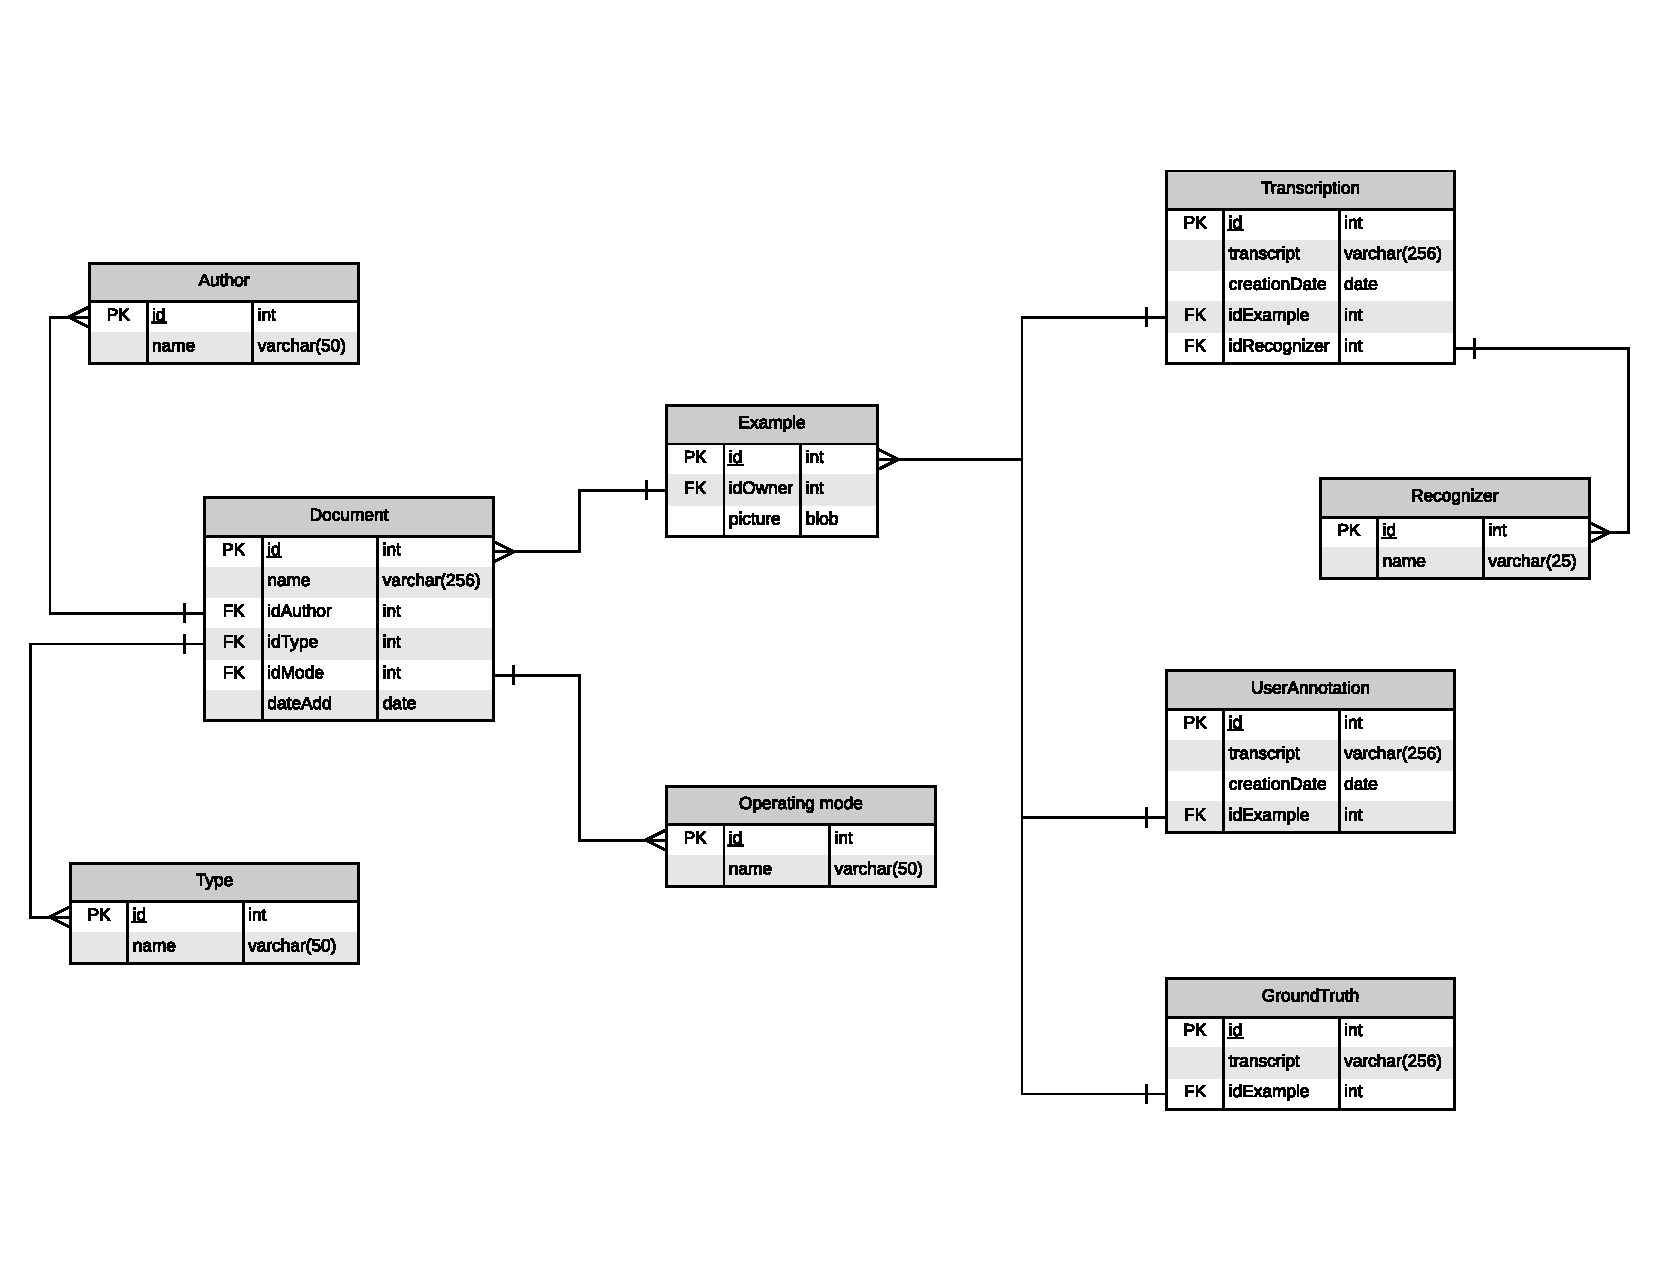
\includegraphics[scale=0.6]{Modele_entite_association.pdf}
\end{center}
\end{mdframed}

\paragraph{}

Les tables \textbf{Author}, \textbf{Type} et \textbf{Operating Mode} permettent
de stocker les informations concernant les auteurs des documents, le type des
documents ainsi que le mode dans lequel on se trouve (mode apprentissage ou
mode évaluation). La table \textbf{Document} contient toutes les informations
concernant un document, à savoir : son nom, son auteur, son type, le mode auquel
il appartient, ainsi que sa date d’ajout à la base.

\paragraph{}
Nos imagettes seront stockées dans des dossiers à côté de la base de données.
Elles seront donc référencées par la base de données grâce à leur chemin (par
exemple \texttt{/home/user/MesImagettes/imagette1.jpg}) dans la table
\textbf{Example}. Cette table contient en plus une référence vers le document
d’origine.

\paragraph{}

Les trois tables suivantes (\textbf{Transcription}, \textbf{UserAnnotation},
\textbf{GroundTruth}) servent à lier les imagettes avec leur transcription.
Dans la table \textbf{GroundTruth}, on enregistre l’identifiant de l’imagette
ainsi que sa vérité-terrain. Dans la table \textbf{UserAnnotation}, on
enregistre la même chose mais, en plus, la date de création de cette
vérité-terrain qui aura été ajoutée par un utilisateur. Enfin, dans la
table \textbf{Transcription}, on enregistre les mêmes informations que dans
la table \textbf{UserAnnotation}, sauf que, cette fois-ci, la transcription
aura été donnée par un reconnaisseur d’écriture manuscrite représenté dans
la table \textbf{Recognizer}.

\paragraph{}

La BDD sera gérée depuis le contrôleur via une classe \textbf{Database}
contenant des méthodes pour communiquer avec elle. Une première version du
diagramme de classes de cette partie est illustré en figure 12.

\paragraph{}

\begin{mdframed}[frametitle={Figure 13 : Diagramme de classes de l'interface avec la BDD}, innerbottommargin=10]
\begin{center}
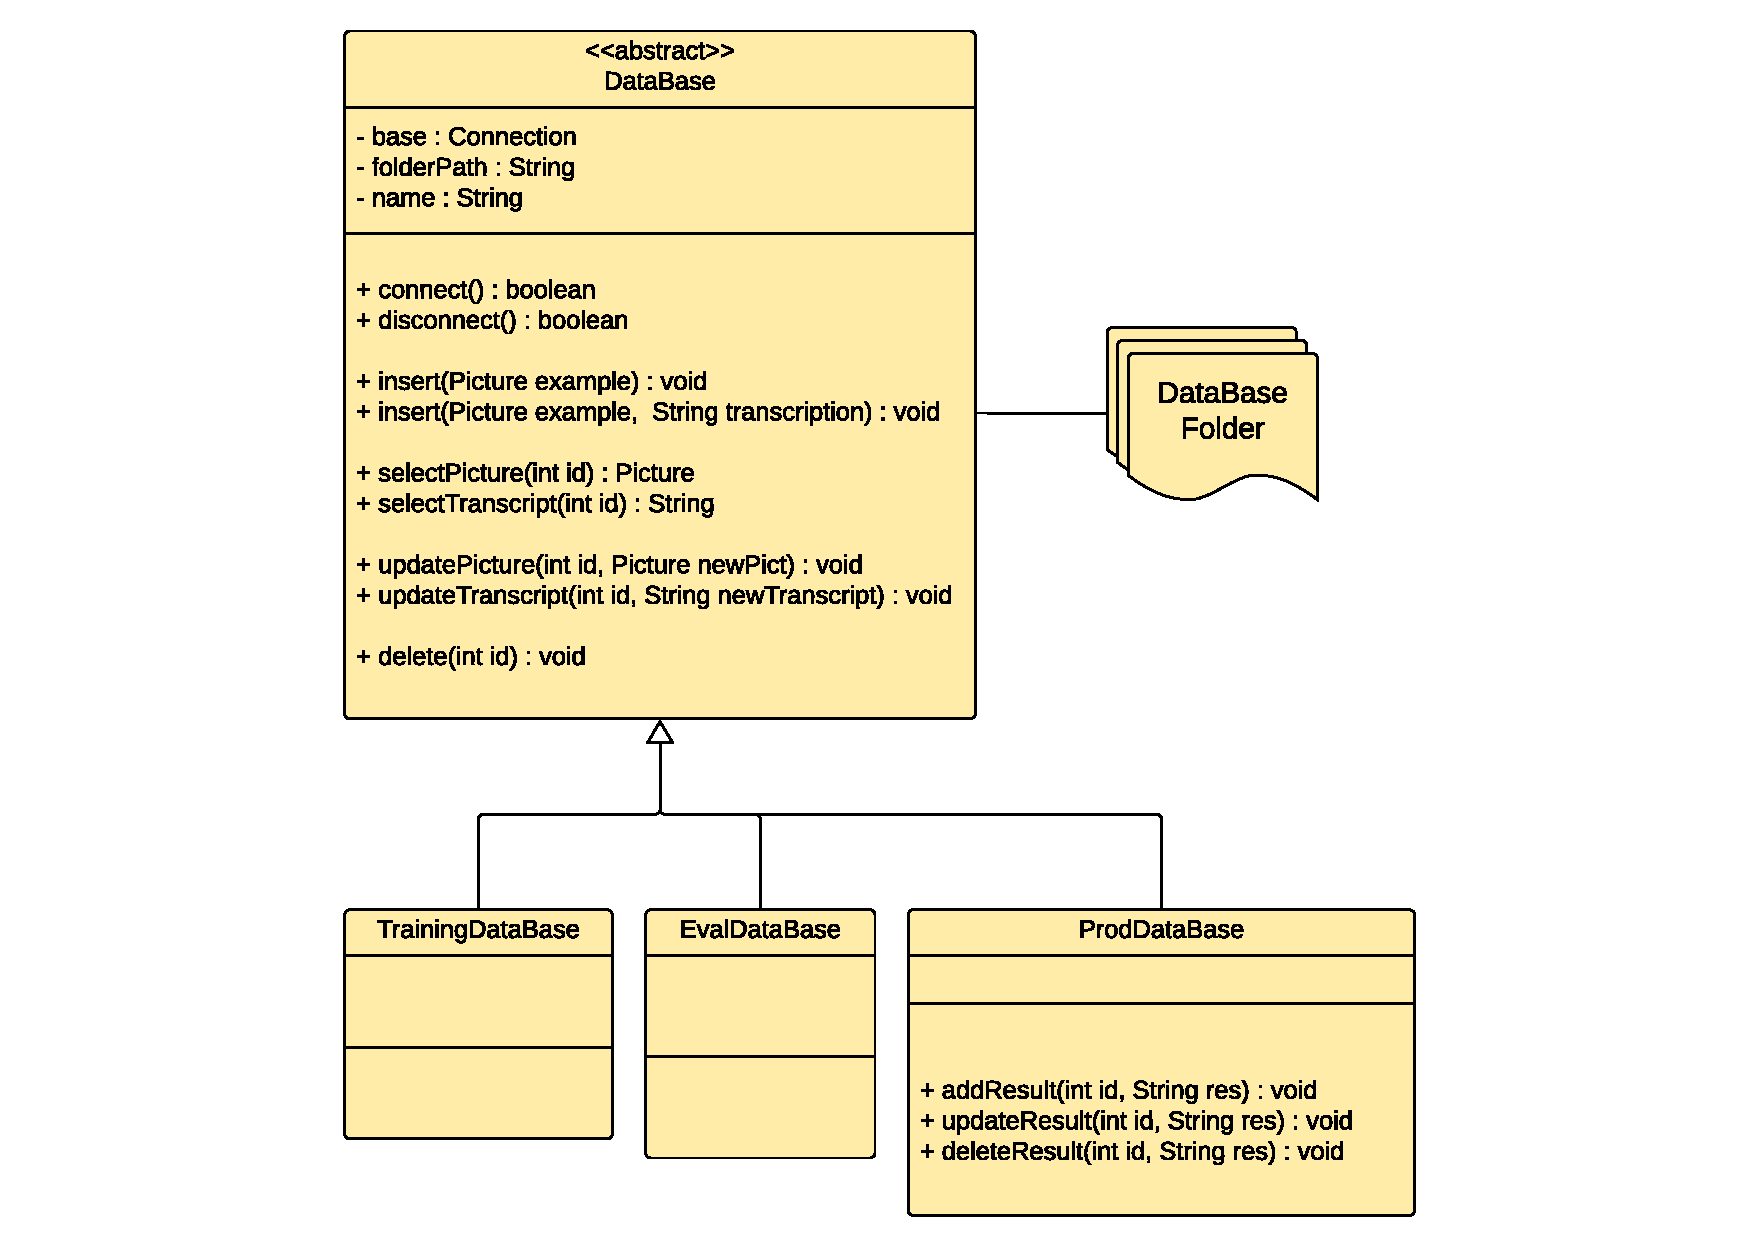
\includegraphics[scale=0.5]{bdd.pdf}
\end{center}
\end{mdframed}

\paragraph{}

Elle peut se connecter à la BDD et se déconnecter, ajouter des exemples avec
et sans transcription, extraire des exemples et les modifier ou les supprimer.
A chaque mode est associé une classe héritant de la classe \textbf{Database}
et possédant les méthodes exclusives à ce mode. On obtient ainsi trois
classes, \textbf{TrainingDataBase}, \textbf{EvalDataBase} et
\textbf{ProdDataBase}, cette dernière classe pouvant également ajouter les
résultats du système de reconnaissance d'écriture manuscrite.

\subsection{Interface avec le système de reconnaissance}

Le programme qui se chargera de faire l’interface entre les données de notre
base et un reconnaisseur sera assez simple. Il se contentera d’extraire les
données pertinentes de la base pour ensuite les convertir au bon format.
Son architecture générale est illustrée par le schéma ci-dessous.

\newpage

\begin{mdframed}[frametitle={Figure 14 : Diagramme de classes de l'interface avec le système de reconnaissance d'écriture manuscrite}, innerbottommargin=10]
\begin{center}
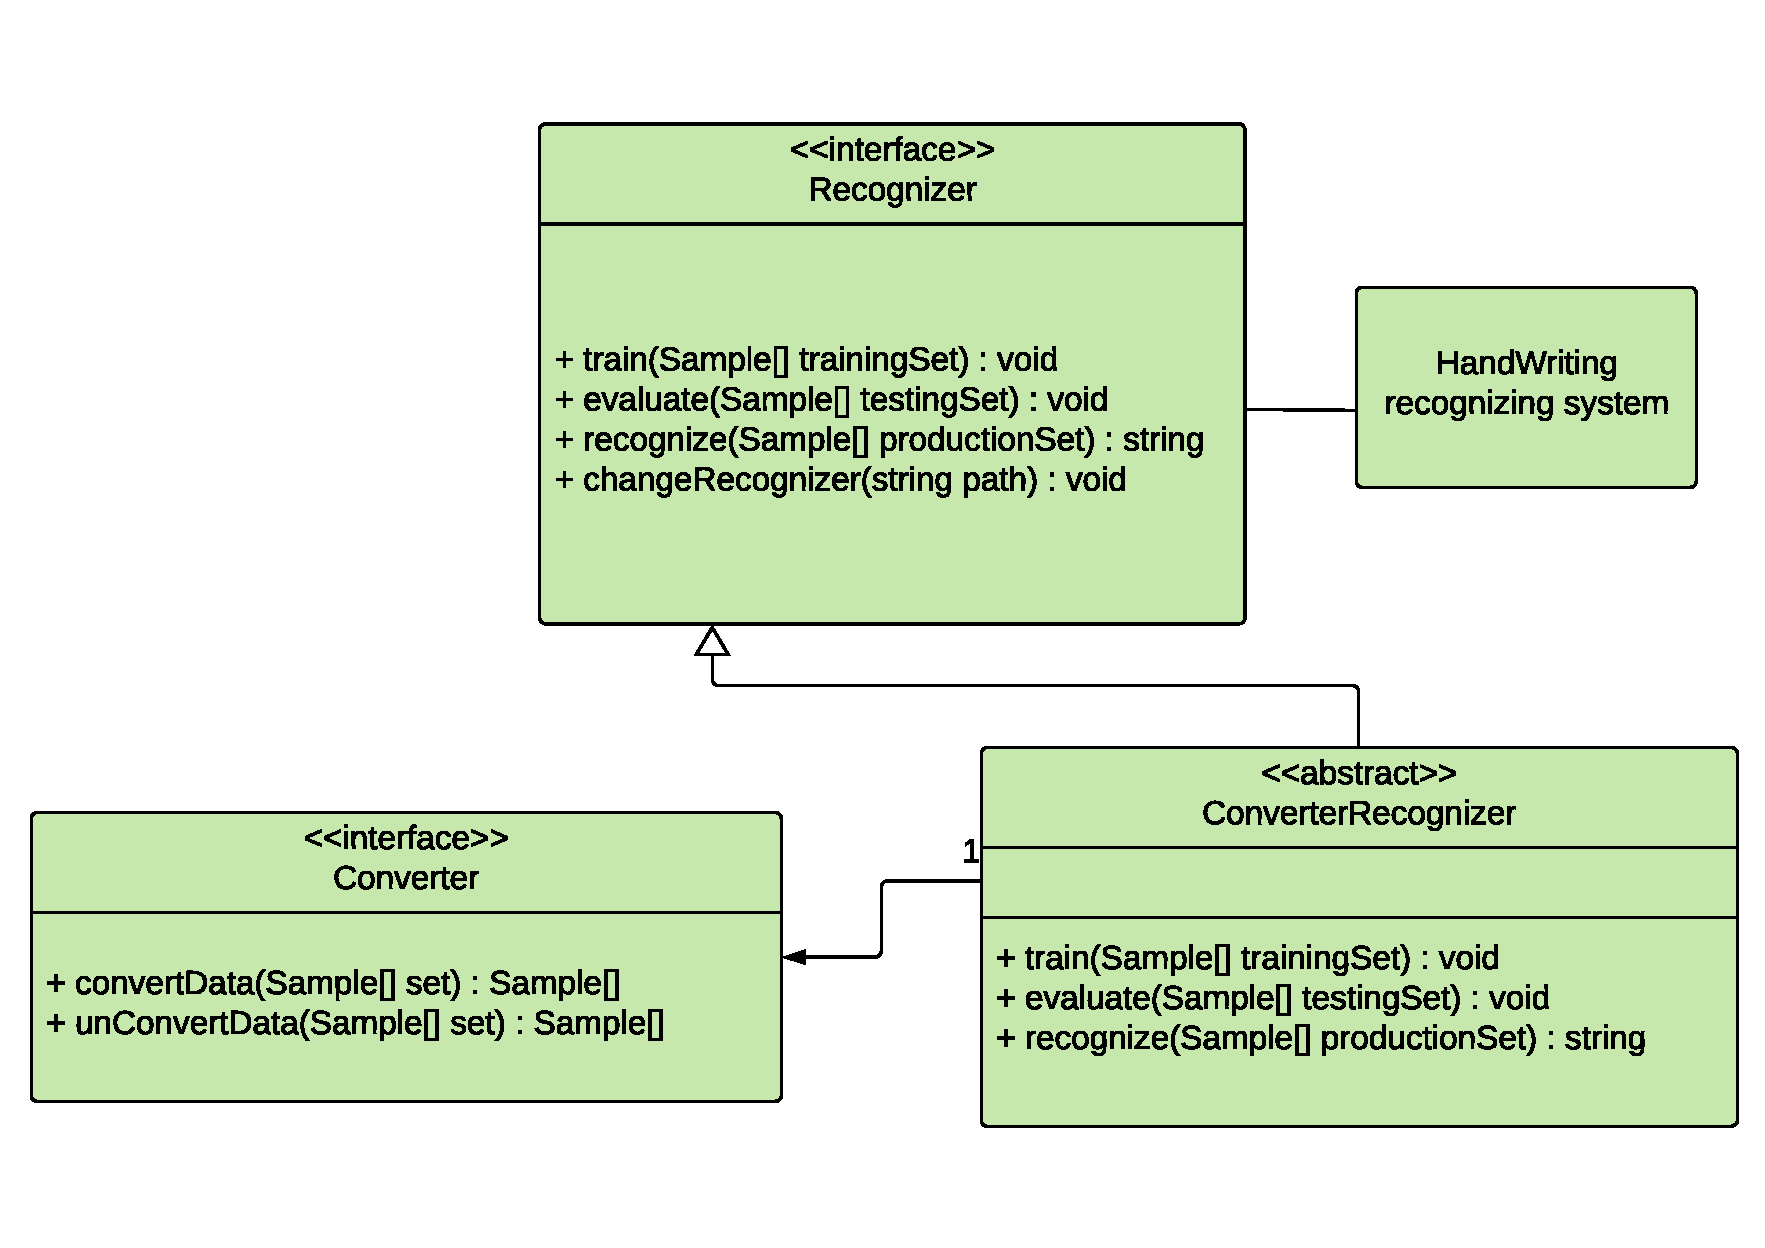
\includegraphics[scale=0.5]{interface-reconnaisseur.pdf}
\end{center}
\end{mdframed}

\paragraph{}
Une interface appelée \textbf{Recognizer} est associée au système de
reconnaissance d’écriture manuscrite. cette interface possède des méthodes
pour fournir des données d'entraînement ou  évaluer le reconnaisseur, ou pour lui faire reconnaître
des jeux de données. Un ensemble d’exemples est envoyé au reconnaisseur qui
les traite. Si les données nécessitent d’être converties, une classe
\textbf{ConverterRecognizer} héritant de cette interface peut être utilisée.
Elle possède en attribut une classe \textbf{Converter} pouvant exécuter des
méthodes pour convertir les exemples d’un format à un autre. Ces méthodes de
la classe \textbf{Converter} seront appelées par les méthodes d’entraînement,
d’évaluation, etc, en amont du traitement qu’elles doivent effectuer.

\paragraph{}
Au cours du développement, des implémentations de ces interfaces ou classes
abstraites seront réalisées.

\subsection{Interface Homme-Machine}

L’IHM sera constituée de cinq pages différentes :
\begin{itemize}
\item une page d’accueil qui permet à l’utilisateur de sélectionner le document
sur lequel il souhaite travailler, ainsi que le mode d’édition des annotations
de son choix ;
\item une page correspondant au mode 1 de l’édition des annotations
(sans vérité-terrain au préalable ou avec des vérités-terrain manquantes) où
l’utilisateur rentre manuellement toutes les annotations ;
\item une page correspondant au mode 2 (correction des transcriptions de l’IA)
où l’utilisateur vérifie le travail de l’IA et corrige les fautes si besoin ;
\item une page correspondant au mode 3 (validation finale) où les
vérités-terrain ont été préalablement validées par l’utilisateur. Cette page
propose une lecture rapide pour corriger les éventuelles erreurs restantes ;
\item une page d’édition des zones où l’utilisateur peut définir et modifier
les différentes zones qui découpent le manuscrit.
\end{itemize}

\paragraph{}
Les cinq pages communiquent entre elles selon le schéma suivant :

\paragraph{}
\begin{mdframed}[frametitle={Figure 15 : Hiérarchie entre les pages}, innerbottommargin=10]
\begin{center}
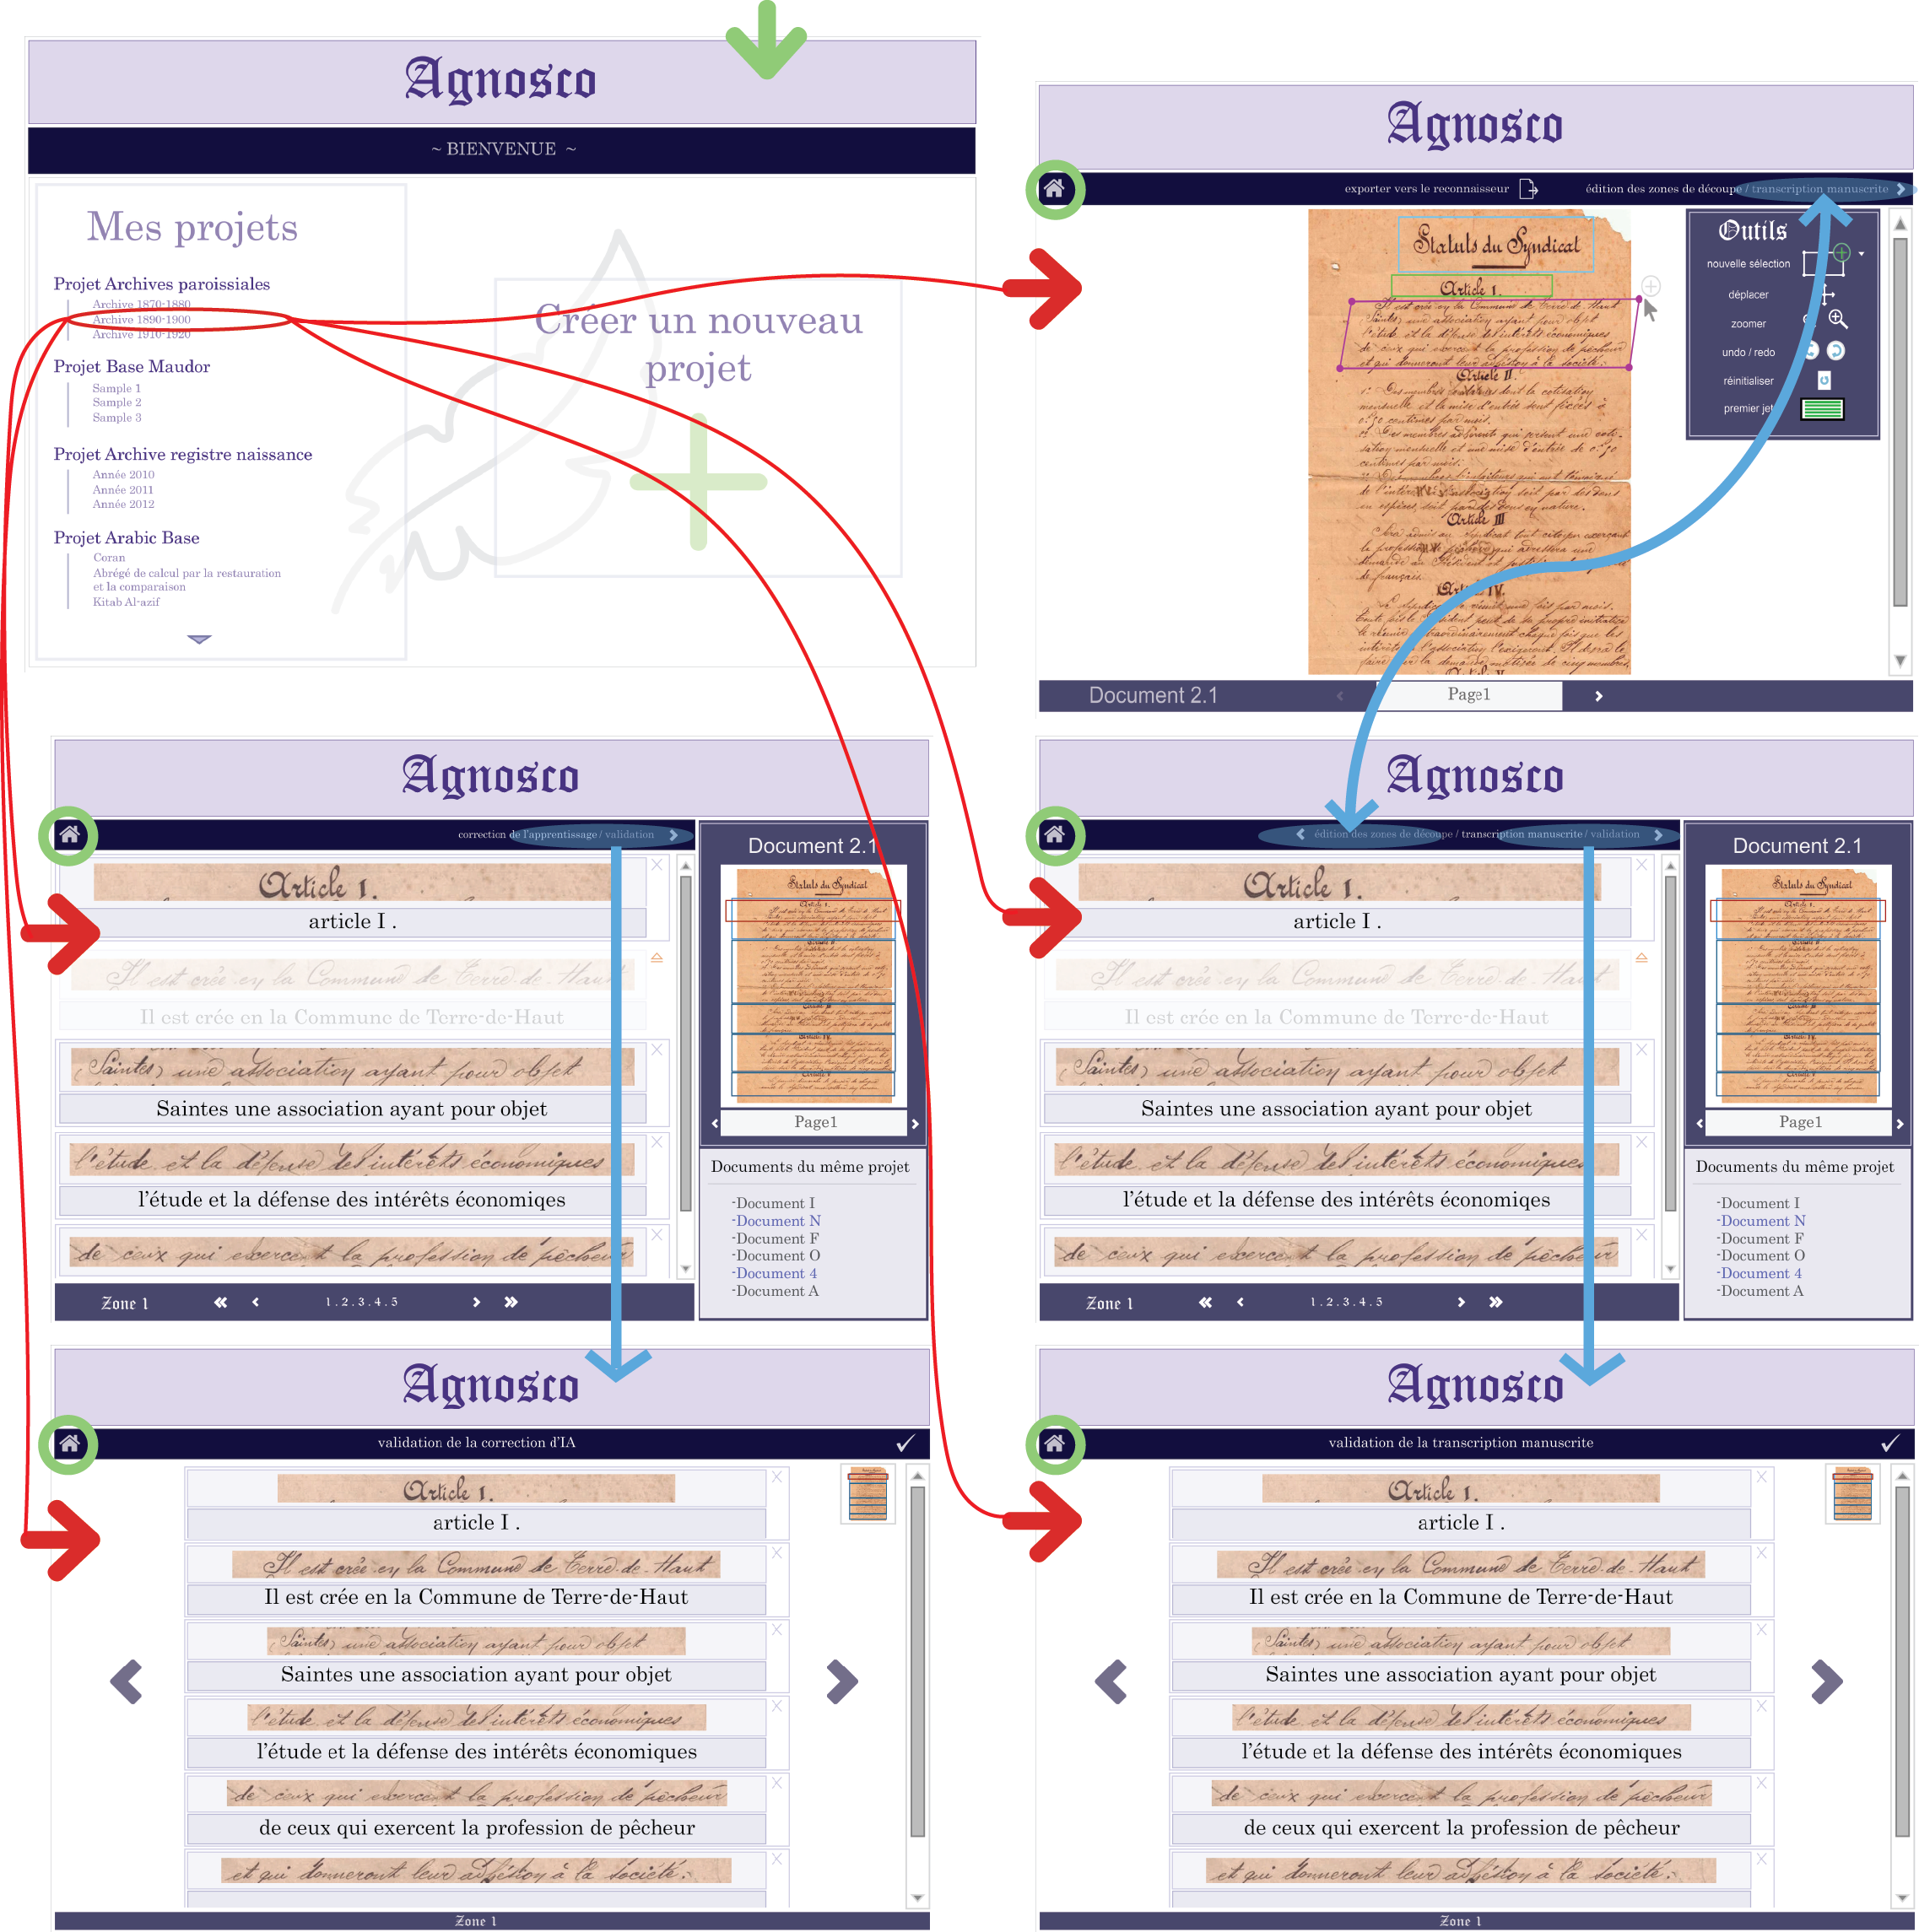
\includegraphics[scale=0.6]{ihm6.png}
\end{center}
\end{mdframed}

L’interface est orientée web, en JavaScript pour une plus grande accessibilité 
et une meilleure portabilité. Ce choix a également pour but de faciliter 
l’évolution de l’application vers une solution multi-utilisateurs distants, 
où plusieurs personnes s‘y connecteraient via Internet.

\section{Interactions}

Tous les modules présentés dans la partie précédente doivent interagir entre
eux à plusieurs niveaux. Un contrôleur général permet de gérer la communication
et la coopération des différents modules. Une première architecture de celui-ci
est visible sur la figure 15.

\paragraph{}
Le diagramme reste général et n’entre pas dans les détails de l’implémentation
qui restent encore à définir. Les couleurs correspondant aux couleurs des
parties expliquées sur la figure 1.

\paragraph{}
Le contrôleur possède une classe correspondant à la partie préparation des
données (en bleu). Celle-ci contient des méthodes pour générer des exemples
à ajouter à la BDD. Une autre classe (en jaune) permet de communiquer avec
la BDD. Elle contient une méthode pour se connecter à la BDD, et d’autres pour
envoyer, recevoir ou modifier des données stockées. Une dernière classe
(partie en vert) permet ensuite de faire le lien avec le système de
reconnaissance d’écriture manuscrite. Elle contient des méthodes pour lancer
l’apprentissage ou l’évaluation du reconnaisseur ou pour l’utiliser sur un
exemple en mode production. Le contrôleur communique enfin avec l’IHM pour
traiter les demandes de l’utilisateur et lui renvoyer les images et
transcriptions. L’IHM est traitée par un serveur web.

\newpage

\begin{mdframed}[frametitle={Figure 16 : Diagramme de classes du contrôleur}, innerbottommargin=10]
\begin{center}
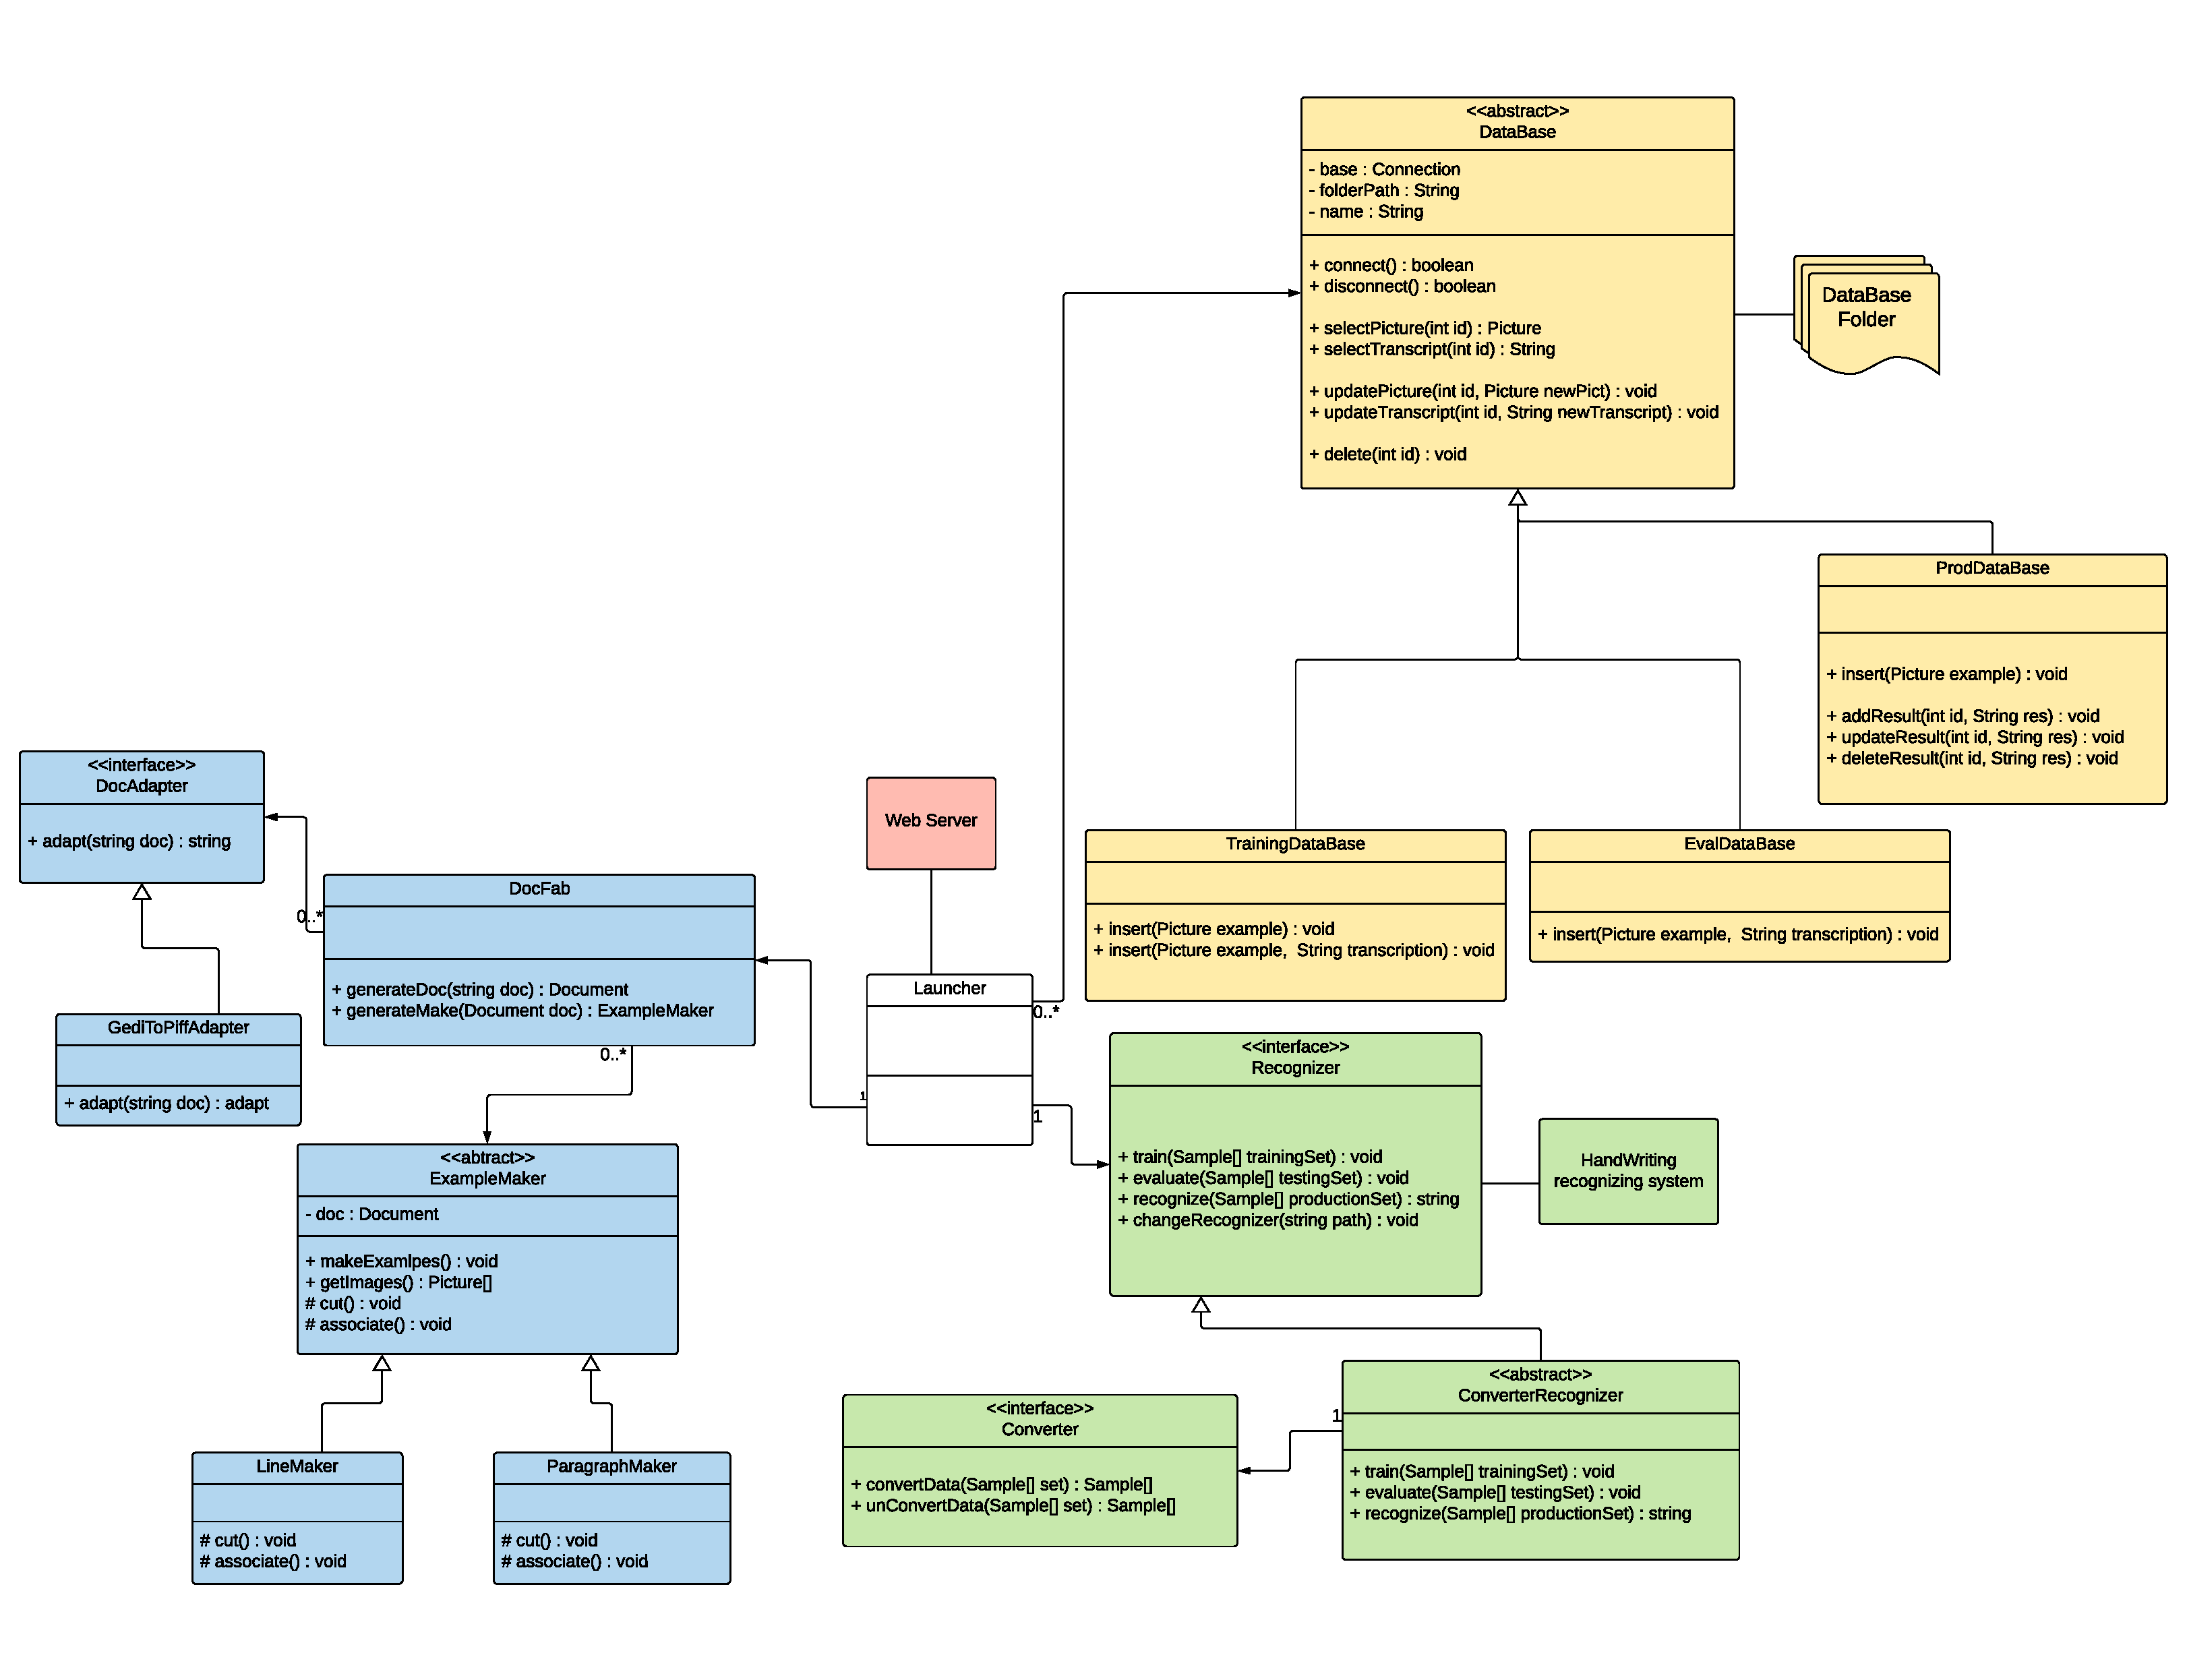
\includegraphics[scale=0.3]{Specifications.pdf}
\end{center}
\end{mdframed}
